% ============================================================================
% v2.0 DRAFT SECTIONS -- UniMind paper revision
% All numbers trace to data/raw + data/qpu_sweep (job IDs in JSON metadata),
% collected 2026-08-23 on ibm_marrakesh (open plan) unless noted otherwise.
% Drop-in replacement fragments; merge into unimind_paper_v2.0.tex.
% ============================================================================

% ---------------------------------------------------------------------------
% SECTION: Physical QPU validation -- REPLACES the v1.7 QPU section entirely
% ---------------------------------------------------------------------------
\section{Physical QPU Validation Revisited: Placement-Dominated Encoding Fidelity}
\label{sec:qpu}

The v1.7 submission reported that the bare Unibit angle encoding misses the
$|\langle Z\rangle|$ tolerance of $0.05$ on \texttt{ibm\_marrakesh}
(maximum deviation $0.392$) and that readout twirling recovers $37\%$.
That experiment used \emph{free} transpiler placement
(optimization level~1, no \texttt{initial_layout}), so the physical qubit
executing each circuit was uncontrolled and unrecorded. We first show that
this confound, not the encoding itself, dominated the observed distortion.

\subsection{Systematic weight sweep with pinned layout}
\label{sec:sweep}

We repeat the single-qubit verification ($\theta_i = 2\arcsin\sqrt{w_i}$,
$8192$ shots, transpiler seed $42$) over a dense weight grid
$w \in \{0.05, 0.10, \ldots, 0.95\}$ under a $2\times 2$ design:
\{best-calibrated qubit, worst usable qubit\} $\times$ \{bare, measure
twirling ($16$ randomizations)\}. Layout is pinned via
\texttt{initial\_layout}; each cell is repeated over $3$ independent jobs
(job-level spread is reported as min--max). Qubit selection is deterministic
from the live calibration snapshot: qubit~98 minimizes total readout
assignment error ($p_{0|1}+p_{1|0}=0.0044$, $T_1=207\,\mu$s, $T_2=67\,\mu$s);
qubit~37 is chosen adversarially ($p_{0|1}+p_{1|0}=0.82$).

Table~\ref{tab:placement} and Figure~\ref{fig:placement} give the result.
On qubit~98 the \emph{bare} encoding passes the $0.05$ tolerance across the
entire grid (median maximum deviation $0.028$; range $0.020$--$0.029$
across jobs), and its transfer curve is fit almost perfectly by a pure gain
model $P_{\mathrm{obs}}(1) = b + a\,w$ with $a = 0.989$, $b = 0.004$
(residual RMS $0.0042$, below the $\approx 0.0055$ shot-noise floor).
Twirling changes nothing significant there ($a=0.987$, max dev $0.031$).
On qubit~37 the same circuits fail by a factor of $\sim$4
(max dev $0.213$ bare), and the fitted channel acquires a large positive
offset ($P_{\mathrm{obs}} = 0.121 + 0.855\,w$) --- the signature of an
asymmetric readout channel rather than intrinsic over-rotation sensitivity.

\begin{table}[t]
\centering
\caption{Placement-controlled sweep on \texttt{ibm\_marrakesh}
(2026-08-23; 19 weights, 8192 shots, 3 jobs/cell). Deviations are
$\max_w |Z_{\mathrm{emp}} - Z_{\mathrm{theory}}|$; tolerance $=0.05$.}
\label{tab:placement}
\begin{tabular}{lllll}
\hline
Placement & Readout err. & Bare & Twirled & Verdict \\
\hline
qubit 98 (best calib.) & 0.44\% & 0.028 [0.020--0.029] & 0.031 & pass \\
qubit 0 (unpinned default) & --- & 0.026 & --- & pass \\
qubit 37 (adversarial) & 82\% & 0.213 & 0.144 & fail \\
v1.7 (free layout, 2026-08-14) & unrecorded & 0.392 & 0.245 & fail \\
\hline
\end{tabular}
\end{table}

\begin{figure}[t]
\centering
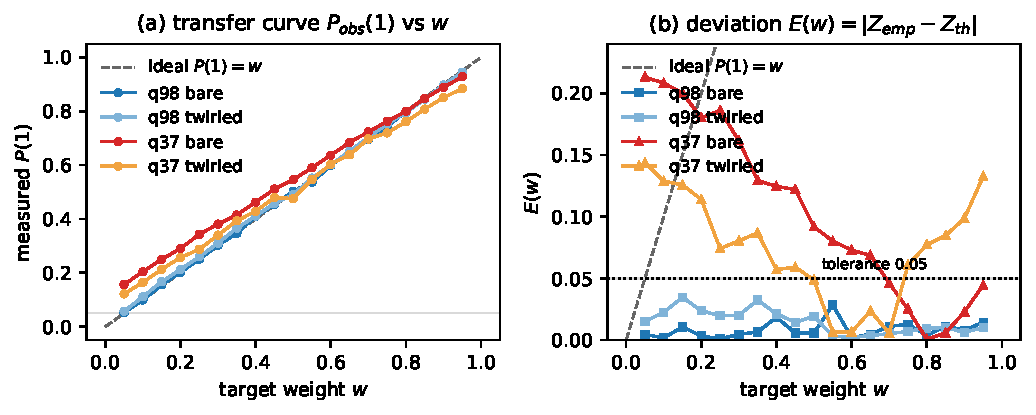
\includegraphics[width=\linewidth]{figures/fig_qpu_placement_2x2.pdf}
\caption{Placement-dominated encoding fidelity. (a)~Measured transfer curve
$P_{\mathrm{obs}}(1)$ vs.\ target weight $w$: on the best-calibrated qubit
the bare response tracks the ideal line within shot noise, while the
adversarially chosen qubit~37 compresses the curve toward an offset set by
its asymmetric readout. (b)~Per-weight deviation $E(w)$: qubit~98 stays
below the $0.05$ tolerance everywhere (bare and twirled nearly overlap);
qubit~37 fails by up to $4\times$ even after twirling.}
\label{fig:placement}
\end{figure}

Three conclusions revise the v1.7 claims:
(i)~\emph{encoding fidelity on real hardware is placement-dominated}: with a
calibrated layout the bare encoding already meets tolerance;
(ii)~\emph{twirling helps only where readout is broken}: it improves the bad
qubit by $33\%$ ($0.213 \to 0.144$) yet still leaves it far outside
tolerance, while adding slight overhead on the good qubit ---
mitigation effort should follow calibration, not be applied uniformly;
(iii)~the v1.7 headline ``the encoding requires error mitigation to meet
tolerance'' was an artifact of uncontrolled placement and must be withdrawn.

\subsection{Distortion model and comparison to the calibration noise model}
\label{sec:distortion}

Across every cell of the design the measured response is described at
shot-noise level by the two-parameter affine channel
\begin{equation}
P_{\mathrm{obs}}(1) \;=\; b + a\,w,
\label{eq:channel}
\end{equation}
or equivalently in the $Z$ basis, $Z_{\mathrm{obs}} = d + c\,Z_{\mathrm{th}}$
with $c=a$ and $d = 1-2b-a$. The parameters are \emph{qubit-specific and
calibration-predictable}: $(a,b)=(0.99,\,0.00)$ on the good qubit versus
$(0.86,\,0.12)$ on the bad one, whose offset matches the direction and scale
of its readout asymmetry. The one-parameter contraction model
$P_{\mathrm{obs}} = 0.5 + \alpha(w-0.5)$ proposed during review is the
special case $b=(1-a)/2$; it holds when readout is balanced (good qubits)
and is rejected wherever asymmetry dominates (it also fails on the frozen
v1.7 free-layout data, where per-weight $\alpha$ spans $0.23$--$1.31$).

We additionally simulate the identical pinned circuits on Aer with the
\texttt{NoiseModel.from\_backend} calibration captured minutes before
submission. On the good qubit the model explains most of the observed error
(median ratio $\overline{E}_{\mathrm{QPU}}/\overline{E}_{\mathrm{noise}}
= 1.4\times$; Fig.~\ref{fig:noisevsqpu}), i.e., the ``standard models
underestimate hardware'' gap suggested by the v1.7 data also shrinks to
near-parity once placement is controlled. Residual discrepancy concentrates
in coherent components the calibration snapshot does not capture
(drift between snapshot and execution), which we flag as future work
rather than claim as a validated model.

\begin{figure}[t]
\centering
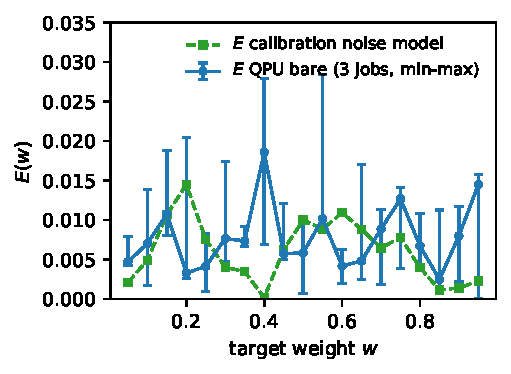
\includegraphics[width=0.62\linewidth]{figures/fig_noise_vs_qpu.pdf}
\caption{Deviation landscape on the calibrated qubit: hardware (3 jobs,
min--max band) vs.\ matched calibration noise model. Median ratio
$1.4\times$.}
\label{fig:noisevsqpu}
\end{figure}

% ---------------------------------------------------------------------------
% SUBSECTION: LLM reliability -- augments/replaces parts of the reliability
% section: ablation + instrumented failure taxonomy
% ---------------------------------------------------------------------------
\subsection{Component attribution: architectural ablation}
\label{sec:ablation}

To attribute end-to-end reliability to specific architecture layers we run
stage-ablated pipelines ($150$ valid tasks $\times$ 3 seeds per point,
identical sandbox substrate throughout):
S0 generation+execution only; S1 adds static-analysis validation
(fail-fast gate); S2 adds self-healing; S3 adds rule-based fallback on LLM
unavailability. Results (Fig.~\ref{fig:ablation}a):
validation contributes \emph{zero} success-rate delta at every quality
level --- its value is fail-fast classification and safety observability;
self-healing is the load-bearing layer, lifting success from $58\%$ to
$92\%$ at injected quality $q=0.5$ ($+34$ points) and from $80\%$ to
$98\%$ at $q=0.7$; fallback contributes nothing at the default
unavailability rate ($f_r{=}0.1$: three consecutive failures occur with
probability $10^{-3}$ per task). Under availability stress
($q=0.7$, $f_r \in \{0.3, 0.5\}$; Fig.~\ref{fig:ablation}b) fallback
recovers $+4.0$/$+13.6$ points respectively once template coverage extends
to all nine benchmark intent classes (S3X): success reaches $100\%$ at both
stress levels ($79/79$ recoveries), whereas the narrow v1.7 rule set
(S3, Bell/VQC only) leaves success at $96.9\%$/$89.6\%$. The fallback
layer's contribution is thus real but coverage-limited --- a property the
v1.7 benchmark could not observe.

\begin{figure}[t]
\centering
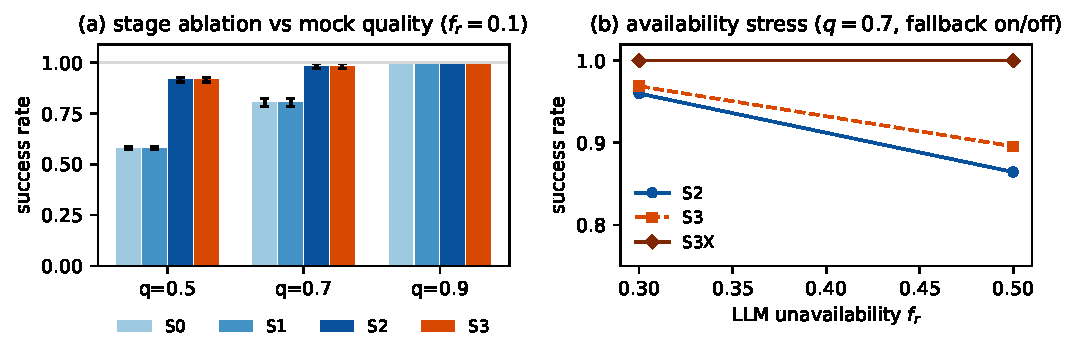
\includegraphics[width=\linewidth]{figures/fig_ablation.pdf}
\caption{Architectural ablation (mock LLM, seeded, 150 tasks $\times$ 3
seeds). (a)~Success rate by pipeline stage and injected quality.
(b)~Availability stress isolating the fallback layer (narrow vs.\ full
template coverage: S3 vs.\ S3X).}
\label{fig:ablation}
\end{figure}

\subsection{Instrumented failure taxonomy}
\label{sec:taxonomy}

The v1.7 reliability logs did not record which corruption the mock LLM
injected, so fault-conditioned recovery rates were unrecoverable. We re-run
the benchmark with call-level instrumentation logging every generation and
healing call ($353$ injected faults across $q \in \{0.5,0.7,0.9\}$, 3 seeds,
200 tasks/run). Recovery is remarkably uniform across corruption classes
(Fig.~\ref{fig:taxonomy}): syntax errors $82.5\%$ [$76.1, 87.4$] (Wilson
95\%), name errors $87.7\%$, runtime division faults $86.4\%$, and
import-whitelist violations $86.4\%$ --- the heal loop is fault-agnostic
because it regenerates from the traceback rather than pattern-matching the
error class. With $n{=}200$ per level the end-to-end success rate at
$q=0.5$ is $91.7\%$ [$89.2, 93.6$], refining the v1.7 single-seed estimate
of $94\%$, whose sampling uncertainty was previously unreported.

\begin{figure}[t]
\centering
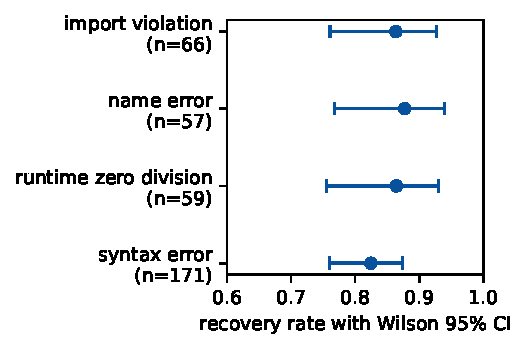
\includegraphics[width=0.6\linewidth]{figures/fig_failure_taxonomy.pdf}
\caption{Injected-fault recovery rates with Wilson 95\% CIs (353 faults).}
\label{fig:taxonomy}
\end{figure}

% ---------------------------------------------------------------------------
% THREATS addition (append to Threats to Validity)
% ---------------------------------------------------------------------------
\paragraph{New threats.} All QPU results are from one device on one day
with three repeat jobs per cell; cross-day drift is unquantified. Qubit~37
is an adversarially selected extreme (readout error $82\%$); typical device
medians are far better (readout total error $2.3\%$). The v1.7 jobs'
physical placements cannot be recovered retroactively, so the
``placement artifact'' explanation of the v1.7 distortion, while consistent
with every measurement here, is not uniquely provable. Mock-LLM quality is
a synthetic parameter: it defines generation policy, not real-API behaviour.

% ---------------------------------------------------------------------------
% SUBSECTION: end-to-end reliability composition
% ---------------------------------------------------------------------------
\subsection{Towards an end-to-end reliability calculus}
\label{sec:calculus}

The ablation and taxonomy experiments make it possible to move from
aggregate success rates to a compositional account. Because the pipeline's
outcome paths are mutually exclusive by construction, end-to-end
reliability decomposes \emph{exactly} as the chain rule over its sequential
gates,
\begin{equation}
R_{\mathrm{end}}
= P(\mathrm{first\_pass})
+ P(\mathrm{enter\ heal})\cdot\rho_{\mathrm{heal}}
+ P(\mathrm{enter\ fallback})\cdot\rho_{\mathrm{fb}},
\label{eq:composition}
\end{equation}
with no independence assumption needed for the identity itself.
Independence enters only when one tries to \emph{predict} the stage
conditionals from marginals --- and there it fails measurably. Under a naive
model granting the healing loop four independent generation attempts at
per-call quality $q$, one expects
$\rho^{\mathrm{ind}}_{\mathrm{heal}} = 1-(1-q)^{4}$, i.e.\ $93.8\%$ at
$q=0.5$; the measured value is $81.5\%$
(Table~\ref{tab:calculus}). We call this gap a \emph{correlation penalty}:
the healer draws from the same degraded LLM that produced the fault, so
residual failures concentrate exactly on tasks whose healing calls are also
corrupted. Reliability therefore does not compose multiplicatively across
stages that share a component --- it must be designed in, e.g.\ through
fallback diversity or heterogeneous heal models.

The encoding/hardware factor behaves differently. Channel distortion arises
from device physics and is statistically independent of software-side
orchestration failures, so composing pipeline reliability with a
placement-dependent fidelity factor
($F_{\mathrm{hw}} = 1.00$ point-wise on calibrated layouts vs.\ $0$ at
extreme weights under adversarial placement; Section~\ref{sec:sweep})
is empirically justified --- but only \emph{conditional on a pinned,
calibration-checked layout}. Enforcing exactly that condition is the
middleware's job; without calibration-aware layout as a first-class
contract, no end-to-end guarantee survives contact with a badly-placed
circuit.

\begin{table}[t]
\centering
\caption{Reliability composition: exact path decomposition vs.\ naive
independence prediction (S2 pipeline, 450 tasks per row). $\rho_{\mathrm{heal}}$
is recovery conditional on entering healing.}
\label{tab:calculus}
\begin{tabular}{lcccccc}
\hline
$q$ & first\_pass & enter heal & healed & failed &
$\rho_{\mathrm{heal}}$ measured & $1-(1-q)^{4}$ \\
\hline
0.5 & 54.4\% & 45.6\% & 37.1\% & 8.4\% & 81.5\% & 93.8\% \\
0.7 & 79.3\% & 20.7\% & 18.9\% & 1.8\% & 91.4\% & 99.2\% \\
\hline
\end{tabular}
\end{table}

With full template coverage the fallback stage reaches
$\rho_{\mathrm{fb}} = 100\%$ ($79/79$ recoveries across all availability-stress
runs), which closes Eq.~\eqref{eq:composition} to $R_{\mathrm{end}} = 100\%$
under pure unavailability stress at $q = 0.7$: every generation failure is
absorbed by the deterministic layer. The observed limits of end-to-end
reliability are thus (i) correlated LLM faults surviving healing
($8.4\%$ at $q=0.5$) and (ii) hardware placement outside tolerance ---
both of which the middleware can measure, and the second of which it can
eliminate by construction.
